\section{Techstack}

\begin{frame}{Techstack}

  \begin{columns}
    \begin{column}{.5\columnwidth}
      \begin{itemize}
        \item Dataset preparation: CDO \cite{schulzweida2019cdo}
        \item algorithm implementation: Julia \cite{gao_julia_2020}
        \item Important libraries:
          \begin{itemize}
            \item (Geo)Makie for Visualisation
            \item KMarkert/EmpiricalOrthogonalFunctions.jl
          \end{itemize}
        
      \end{itemize}  
    \begin{figure}[h]
      \centering
      
\includegraphics[width=.5 \columnwidth]{imglib/julialang_logo.png}
    \end{figure}
    \end{column}
    \begin{column}{.5\columnwidth}
    \begin{figure}[h]
      \centering
      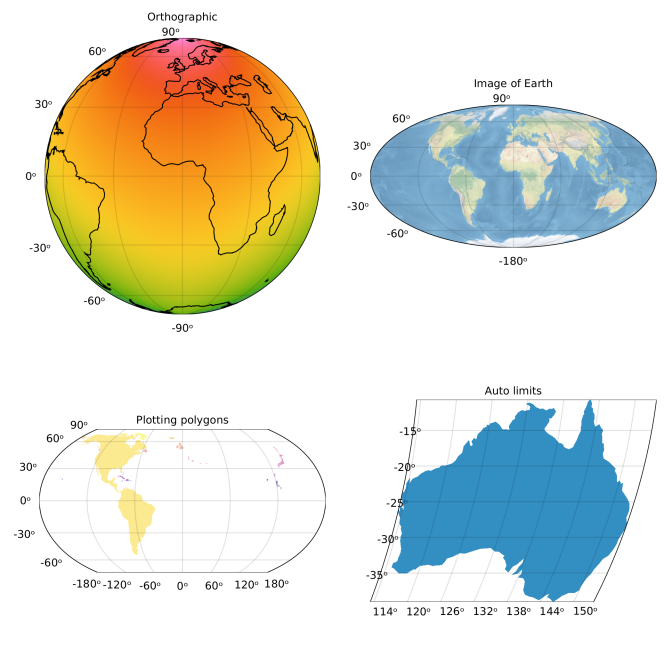
\includegraphics[width=.7 \columnwidth]{imglib/geomakie_examples.png}
    \end{figure}
      
    \end{column}
  \end{columns}
  
\end{frame}
